\documentclass[fleqn, 14pt]{extarticlej}
\oddsidemargin=-1cm
\usepackage[dvipdfm]{graphicx}
\textwidth=18cm
\textheight=23cm
\topmargin=0cm
\headheight=1cm
\headsep=0cm
\footskip=1cm

\def\labelenumi{(\theenumi)}
\def\theenumii{\Alph{enumii}}
\def\theenumiii{(\alph{enumiii})}
\usepackage{comment}
\usepackage{indentfirst}
\begin{document}
%%%%%%%%%%%%%%%%%%%%%%%%%%%%
%% 表題
%%%%%%%%%%%%%%%%%%%%%%%%%%%%
\begin{center}
{\Large {\bf カレンダの整理について}}
\end{center}

\begin{flushright}
2013年6月27日

乃村研究室 河野 達生
\end{flushright}

\section{整理の定義}
整理とは,同種のオブジェクトをなんらかの基準で並べることである.または,無駄なもの,不要なものを処分することである[1].これを整理の定義とする.本資料は,整理の定義にもとづいてカレンダにおける整理について述べる.

\section{カレンダにおける整理}
カレンダにおける整理とは,予定情報を整理することである.予定情報とは,予定の名前,開始時刻,終了時刻をもつものである.次節で予定情報が整理されていない状態と整理されている状態について述べる.

\subsection{予定情報が整理されていない状態}
予定情報の整理されていない状態を以下に述べる.
\begin{enumerate}
	\item 予定を羅列した状態\\
	例を図1に示す.図1は,作成順に予定を羅列した状態である.
\end{enumerate}	

\begin{figure}
  \begin{center}
    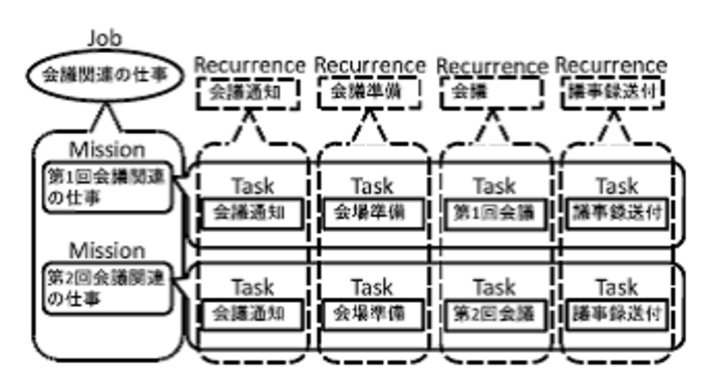
\includegraphics[clip,width=0.7\columnwidth]{zu1.eps}
    \caption{整理されていない状態}
  \end{center}
\end{figure}

\subsection{予定情報が整理されている状態}
予定情報の整理されている状態を以下に述べる.
\begin{enumerate}
	\item 時系列に分類されている.\\
			作成した予定を開始時刻順に並べ替えている状態である.
	
	\item 所属ごとに分類されている.\\
          例を図2に示す.図2は,所属ごとに予定を分類している例である.ユーザが作成した所属に予定を分類している状態である.
 
%     \item TODOの予定が分類されている.\\
%      例を図3に示す.カレンダに記入する予定は期日までにやらなければならないこと(以下,TODOとする.)を記入する場合がある.このため,TODOの予定を分類した状態は整理されていると言える.

	\item 関連する予定が分類されている.\\
          例を図3に示す.図3は,関連する予定を集合として分類している例である.ユーザが作成した集合に関連する予定を分類している状態である.
          
	\item 周期的に発生する予定が分類されている.\\
          例を図4に示す.図4は,周期的に発生する予定を集合として分類している例である.ユーザが作成した集合に周期的に発生する予定を分類している状態である.
          
\end{enumerate}

\begin{figure}
  \begin{center}
    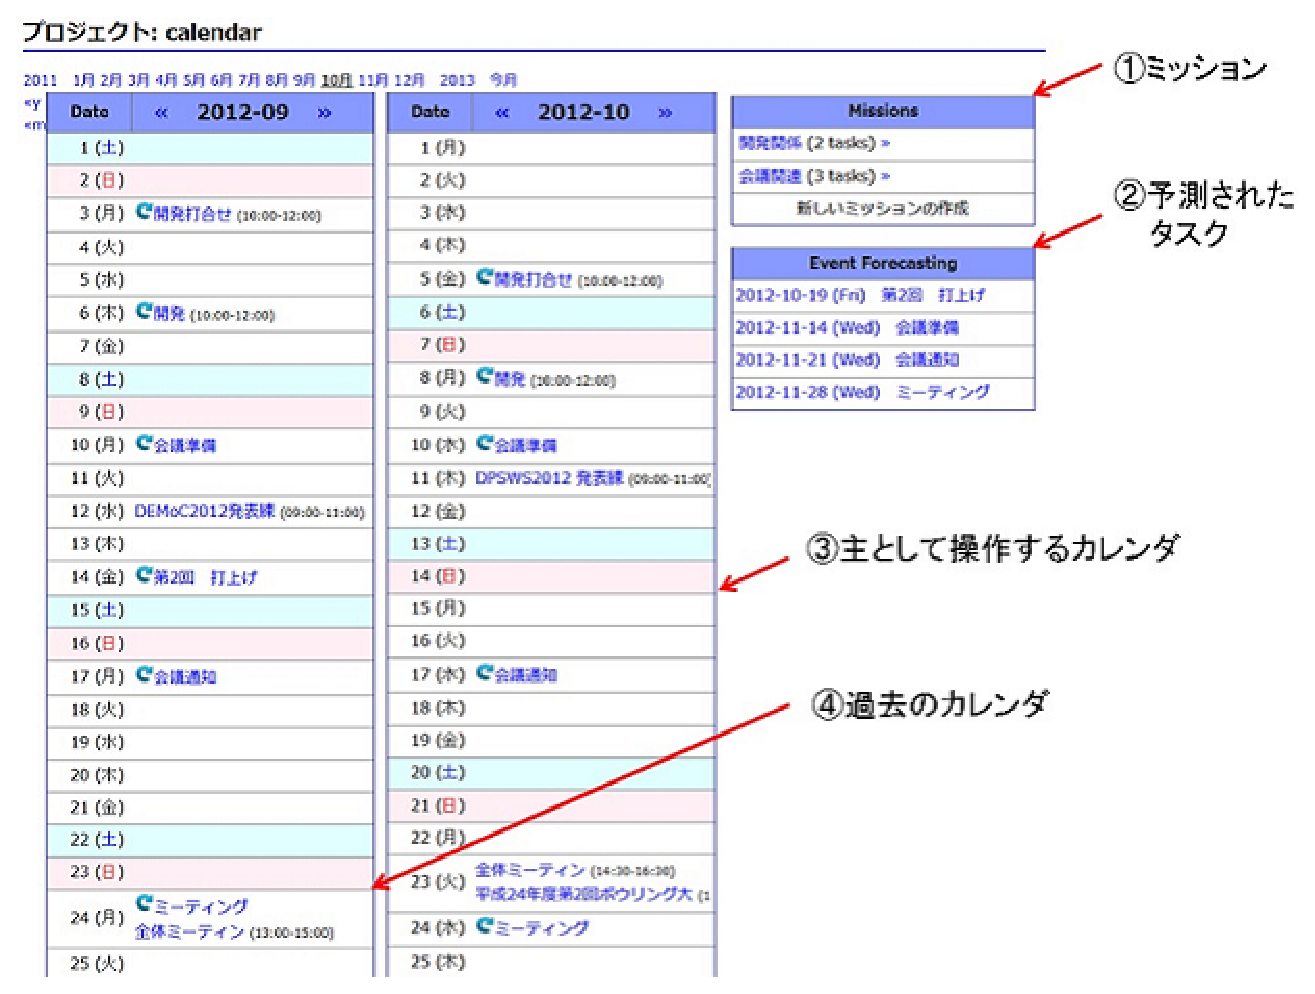
\includegraphics[clip,width=0.7\columnwidth]{zu2.eps}
    \caption{所属ごとに予定を分類した例}
  \end{center}
\end{figure}

\begin{figure}
  \begin{center}
    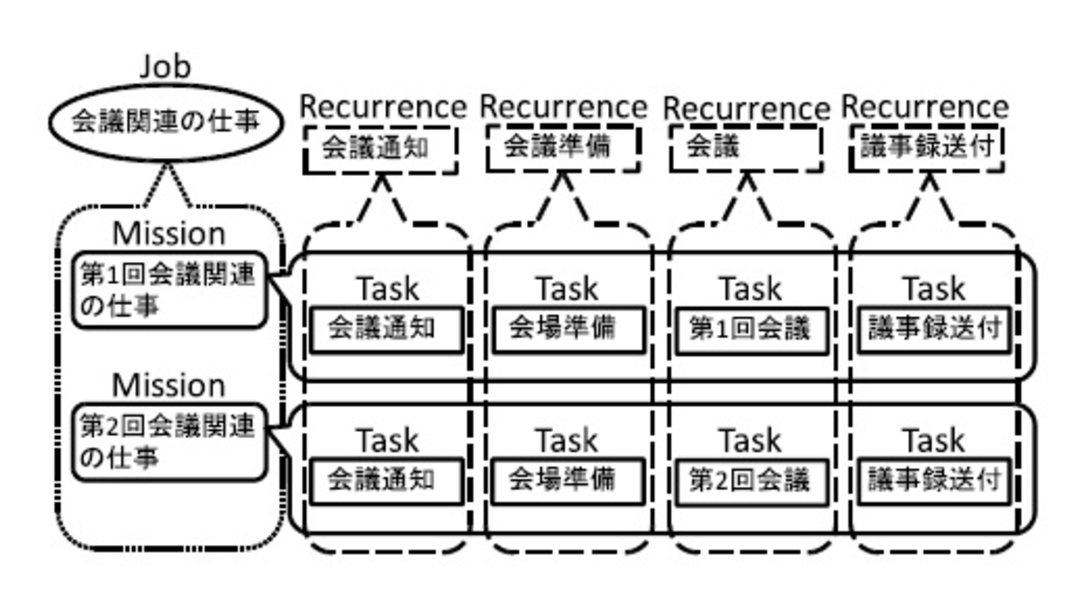
\includegraphics[clip,width=0.7\columnwidth]{zu3.eps}
    \caption{関連する予定が集合として分類した例}
  \end{center}
\end{figure}

\begin{figure}
  \begin{center}
    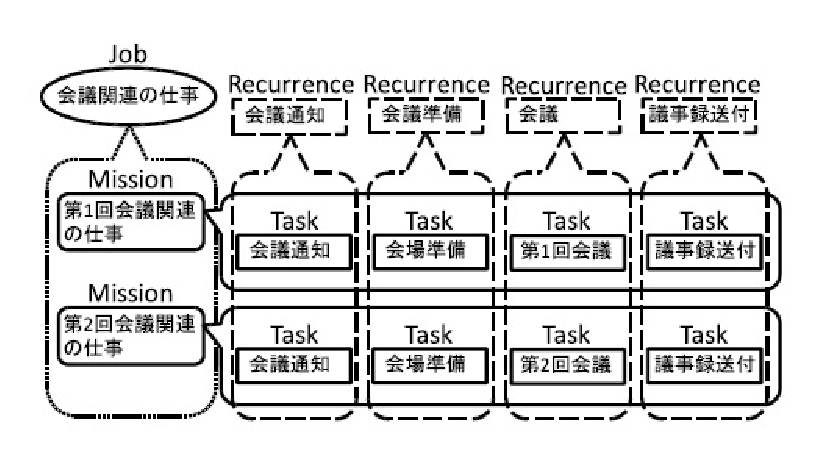
\includegraphics[clip,width=0.7\columnwidth]{zu4.eps}
    \caption{周期的に発生する予定が集合として分類した例}
  \end{center}
\end{figure}

\newpage
\section{カレンダ情報が整理されていない場合の問題点}
予定情報が整理されていないカレンダにおける問題点を以下に述べる.
\begin{enumerate}
	\item 時系列に並んでいない\\
	  特定の日付の決まっている予定を確認したい場合,整理されていない状態では全ての予定を確認しなければならないため,時間がかかる.例を図1を用いて説明する.6月12日の予定を確認したい場合,20個の予定を全て確認しなければ12日の予定を把握できない.

	\item 所属が違う同じ予定名を区別できない.\\
		所属は異なるが予定名が異なるとは限らない.例を図1を用いて説明する.6月1日と6月7日に「打上げ」の予定があるが,この「打上げ」はプライベートに所属する予定か研究室に所属する予定か区別が困難になる.
		
	\item 関連する予定を把握できない.\\
		整理されていない状態から関連する予定を探す場合,必ずしも関連する予定が付近に作成されることはない.このため,関連する予定を把握しきれない.例を図1と図3を用いて説明する.図3より「検討打合せ資料提出」と「検討打合せ」は関連する予定として集合を作成できる.しかし,図1ではどの予定が関連する予定であるか把握することはできない.

%	\item 周期的に発生する予定を把握できない.\\
		
	
\end{enumerate}

%特定の日にカレンダに予定を登録した状態のことを指す.時系列に並んでいる状態では,特定の日の予定を把握するには十分である.しかし,過去を振り返り予定を探し出す場合,見落とす可能性がある.このため,時系列に並んだカレンダを整理されていない状態とする.
%カレンダには,ユーザに関する予定が全て記載されているため,ユーザの所属による予定の把握ができない可能性がある.このため,所属別の予定が混合しているカレンダを誠意されていない状態とする.

%\subsubsection{利点}
%\begin{enumerate}
%	\item 所属別の予定を把握したい場合,有用である.
%	\item 関連する予定の集合と作成することで,複数回行われる予定を管理できる.
%	\item 予定が登録されている日を把握していない場合,予定名から検索することができる.
%	\item 予定名があいまいな場合,予定が登録されている日を範囲指定して検索することができる.
%\end{enumerate}

%所属別に予定を表示させる.これにより,ユーザは所属別に予定を把握したい場合に有用である.
%	予定は1回で終わるものと継続して行われるものが存在する.このため,関連する予定で集合を作成することで,
%ユーザが知りたい情報を素早く得ることができる状態である.カレンダシステムには,予定を検索する機能や所属別にカレンダを分ける機能があるものが多い.このため,整理された状態を作成するために整理の手順を次章に説明する.
\section{まとめ}
本資料は,整理の定義にもとづいてカレンダの予定の整理について述べたものである.整理の定義を明確にしたうえで,今後自身の研究対象であるEnCalについて整理を行い,効率良くリカーレンスやミッションを見つけ出す方法を考察し実装する.

\begin{thebibliography}{99}
  \bibitem {book1} 小学館:コトバンク,デジタル大辞泉(オンライン),入手先

\verb|<|http://kotobank.jp/word/\%E6\%95\%B4\%E7\%90\%86\verb|>|(参照2013-06-19).

\end{thebibliography}



\end{document}
